\documentclass[11pt, a4paper]{article}

\usepackage[utf8]{vietnam}
\usepackage{graphicx}
\usepackage{booktabs}
\usepackage{hyperref}
\usepackage{amsmath,amssymb}
\usepackage{enumitem}
\usepackage[top=2cm, bottom=2cm, left=3cm, right=2cm]{geometry}
\graphicspath{{images/}{submissions/tuan2_doquangvinh/images/}}

\begin{document}

\begin{center}
    {\Large \textbf{BÁO CÁO BÀI TẬP TUẦN 2}}\\[0.3em]
    {\large Phân tích các biến thể mã hóa MaxSAT}
\end{center}

\section{Mục tiêu và phương pháp}
Tuần 2 tập trung vào thực hành trên codebase của dự án \href{https://github.com/Viing3107/maxsattrainscheduling}{maxsattrainscheduling} với 4 mục tiêu:
\begin{itemize}
    \item \textbf{Cài đặt môi trường Linux}: Biên dịch thành công file binary \texttt{target/release/ddd} trên môi trường Linux (Ubuntu/WSL2), liên kết đầy đủ các solver ngoài (CaDiCaL, UWrMaxSat, IPAMIR-rs) và Gurobi 13.2
    \item \textbf{Lập trình kỹ thuật mã hóa}: Cài đặt và kiểm thử độc lập bằng Python 2 kỹ thuật chính của bài báo:
    \begin{enumerate}[label = (\roman*)]
        \item Lan truyền cận dưới hành trình tàu (Precedence Propagation)
        \item Mã hóa Sequential-Counter (SC) AMO với ngưỡng $\theta = 6$
    \end{enumerate}
    \item \textbf{Tái hiện thực nghiệm}: Sử dụng các script trong \texttt{quick\_scripts/bench/} để chạy lại thực nghiệm trên 72 bài toán Na Uy (thuộc 3 nhóm: original, track, station) cho 3 dạng hàm mục tiêu (finsteps123, infsteps180, cont)
    \item \textbf{Phân tích và trực quan hóa}: Viết script Python đọc kết quả CSV để tính thời gian giải trung bình và vẽ biểu đồ so sánh 4 cấu hình (MaxSAT-Base, MaxSAT-SC, MaxSAT-Prec, MaxSAT-Default)
\end{itemize}

\section{Kết quả mã hóa}
Với nhóm xung đột có kích thước $n$, mã hóa Pairwise sinh ra $\frac{n \times (n - 1)}{2}$ clauses, trong khi Sequential Counter sinh ra $3n-4$ clause với $n>2$. Do đó, Pairwise đơn giản hơn ở nhóm nhỏ, còn SC tiết kiệm clause khi $n$ tăng. Kết quả thực nghiệm cho thấy với $n \le 6$ thì Pairwise sinh ra ít clause hơn so với Sequential Counter, nhưng từ $n > 6$ thì Sequential Counter lại cho kết quả tốt hơn. Hai công thức mã hóa cùng một ràng buộc AMO và đã được kiểm chứng tính tương đương nghiệm bằng bộ giải Cadical153 thông qua PySAT.
\begin{figure}[ht]
    \centering
    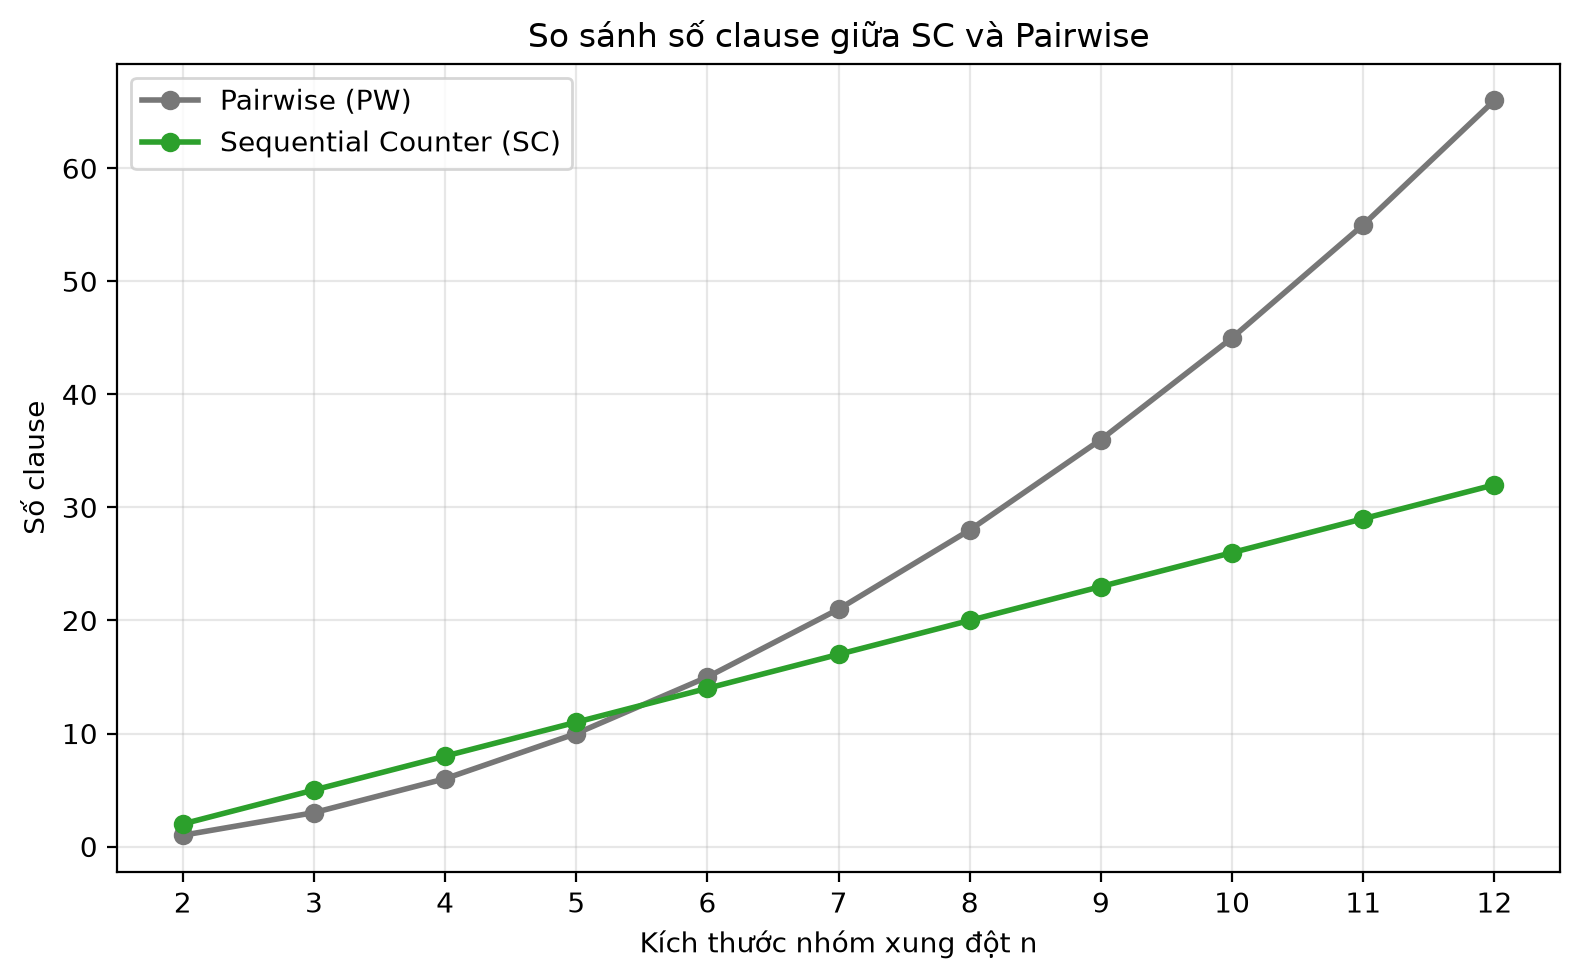
\includegraphics[width=0.78\textwidth]{bai3_clause_sc_vs_pw.png}
    \caption{So sánh số clause giữa mã hóa Pairwise và Sequential Counter.}
    \label{fig:clauses}
\end{figure}

\section{Kết quả thực nghiệm}
\begin{table}[ht]
    \centering
    \small
    \caption{Thời gian giải trung bình (ms)}
    \label{table:sol_time}
    \begin{tabular}{llrrrr}
        \toprule
        Nhóm & Mục tiêu & MS\_Base & MS\_SC & MS\_Prec & \textbf{MS\_Default}\\
        \midrule
        Track & Step & 27.37 & 26.93 & 29.44 & 27.41\\
        Track & Round & 658.70 & 417.86 & 746.49 & \textbf{394.42}\\
        Track & Continuous & 4385.24 & 2025.75 & 1956.00 & \textbf{895.06}\\
        Station & Step & 30.53 & 28.19 & 32.66 & 31.52\\
        Station & Round & 1775.75 & 1668.38 & 1516.08 & \textbf{1064.42}\\
        Station & Continuous & 11501.50 & 11825.21 & 9341.91 & \textbf{8366.86}\\
        \bottomrule
    \end{tabular}
\end{table}

Hình \ref{fig:time} cho thấy bài toán Continuous khó hơn rõ rệt so với Step và
Round. Cấu hình MS\_Default có thời gian thấp nhất ở Round và Continuous trên
cả hai nhóm Track và Station. Ở Step, chênh lệch giữa các cấu hình nhỏ hơn nhiều.

\begin{figure}[ht]
    \centering
    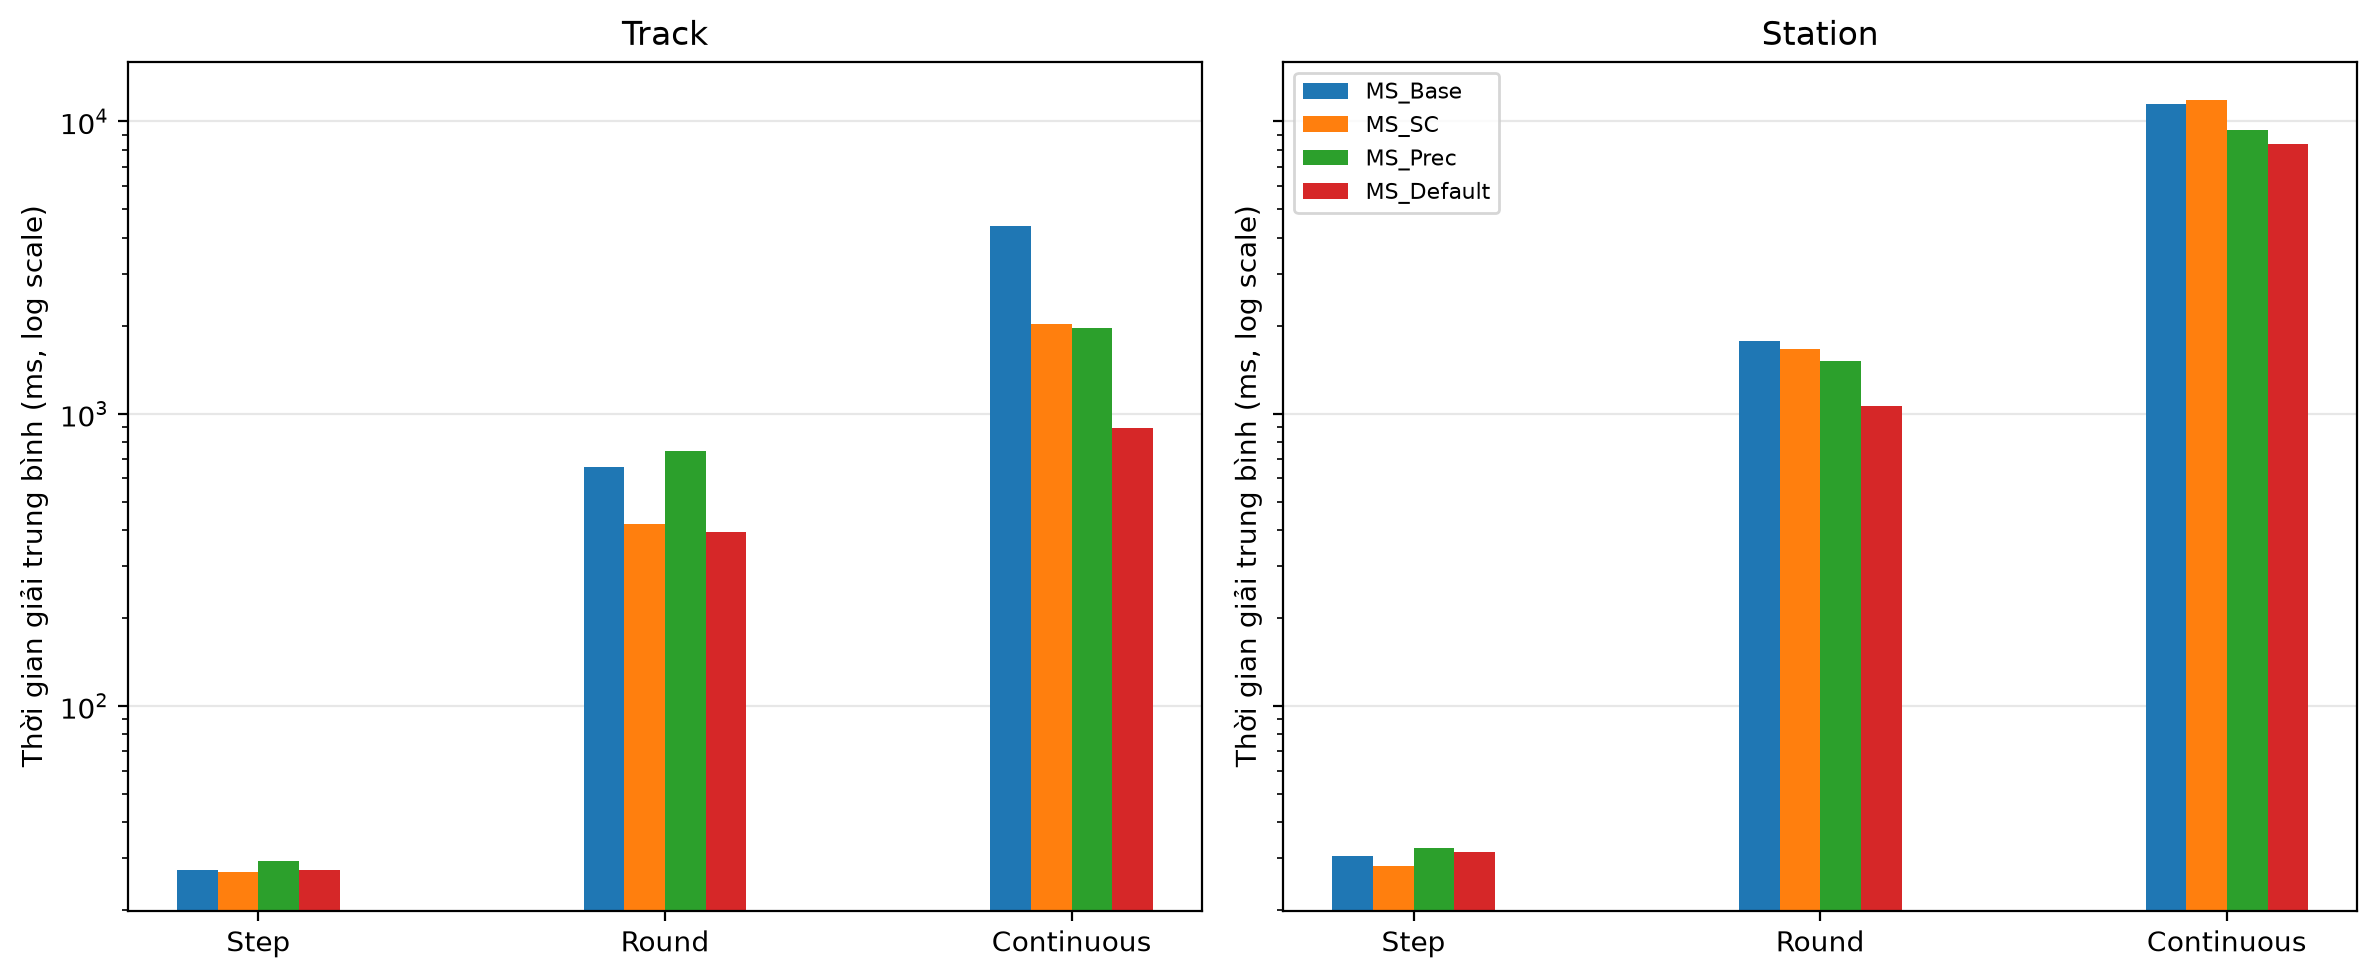
\includegraphics[width=\textwidth]{bai3_average_solve_time.png}
    \caption{So sánh thời gian giải trung bình theo nhóm bài toán.}
    \label{fig:time}
\end{figure}

\section{Kết luận}
Kết quả xác nhận SC có tốc độ tăng số clause tuyến tính, trong khi Pairwise tăng theo bậc hai. Trong các thực nghiệm, việc kết hợp các cải tiến vào MS\_Default cho kết quả ổn định và thường nhanh nhất, đặc biệt trên các mục tiêu Round và Continuous. 

\section{Sản phẩm}
\begin{itemize}
    \item \textbf{Repository Git}: \url{https://github.com/Viing3107/maxsattrainscheduling}
\end{itemize}

\end{document}